
%%%%%%%%%%%%%%%%%%
%                %
% Introduction   %
%                %
\chapter{Introduction}
\label{cp:intro}

%\begin{highlight}
%    \begin{st}
%        General structure with just some dummy text.
%    \end{st} 
%\end{highlight}

\lettrine{M}{obile robots} are a class of robots with the ability to move through the environment~\citep{corke2017robotics}. Most of these robots are power-demanding devices constrained by battery limitations. Whilst such limitations are a common challenge in many areas, they are critical in mobile robots' design and development. They influence the level of autonomy~\citep{seewald2020mechanical}, which in turn is expected to increase in the foreseeable future~\citep{fisher2013verifying}.

To move, mobile robots combine different components which sense and interact with the surrounding environment~\citep{mei2006deployment}. The analysis and interpretation of data originating from these components require energy-demanding heterogeneous computing hardware. Planning an energy-aware path with a power-saving scheduling policy on such hardware is an underrepresented topic in the literature. In fact, many past approaches focus almost exclusively on one of these topics. For instance, some approaches generate an energy-optimized path, despite the energy needed for the computations almost equaling the actuation of some instances of low-energy mobile robots~\citep{sudhakar2020balancing}. Due to the recent advancements in the computational capabilities of mobile hardware, such as the introduction of powerful portable GPUs\findex{GPU}~\citep{rizvi2017general}, the use of computations is expected to increase~\citep{abramov2012real,satria2016real,jaramillo2019visual}. Other approaches provide a power-saving scheduling policy. Yet, actuating a mobile robot requires considerable power over mere calculations~\citep{mei2004energy,mei2005case}.

In this work, we focus on dynamic energy planning by generating an energy-aware plan of the path and a power-saving schedule of the computational tasks. We generate these two aspects simultaneously, exploring their tradeoffs. We demonstrate the approach both in simulation and empirically focusing on aerial mobile robots. These systems share with the broader class of mobile robots very stringent battery limitations. Recharging the battery during normal operation is, however, rarely an option for aerial robots. It would require landing to replace or recharge the battery~\citep{zamanakos2020energy}. They are hence a perfect instance of energy-constrained systems and are the main focus of our analysis.

To achieve dynamic energy planning, we first formulate some autonomous operations for mobile robots that we are studying in \fref{sec:pb-form}{Section}. Such operations often originate from mobile robotics use-case as precision agriculture, search and rescue, payload delivery, transportation, and many others. We focus on the first two applied to the aerial robotics context. We then build an energy model to predict future energy consumption in \fref{cp:model}{Chapter}. We estimate the coefficients of the model using robust estimation techniques in \fref{cp:est}{Chapter}. Later, we derive an optimal configuration of the path and computations use data-driven control\findex{data-driven control} and other modern optimal control techniques in \fref{cp:opt}{Chapter}. Here some estimates are made from sensors' data and used to derive an optimal control action. We use such optimal control for guidance and scheduling of the aerial robot in \fref{cp:gd}{Chapter}. The guidance moves physically the robot; the scheduling defines the granularity of the tasks being executed in flight.

\begin{figure}[t]
  \centering
  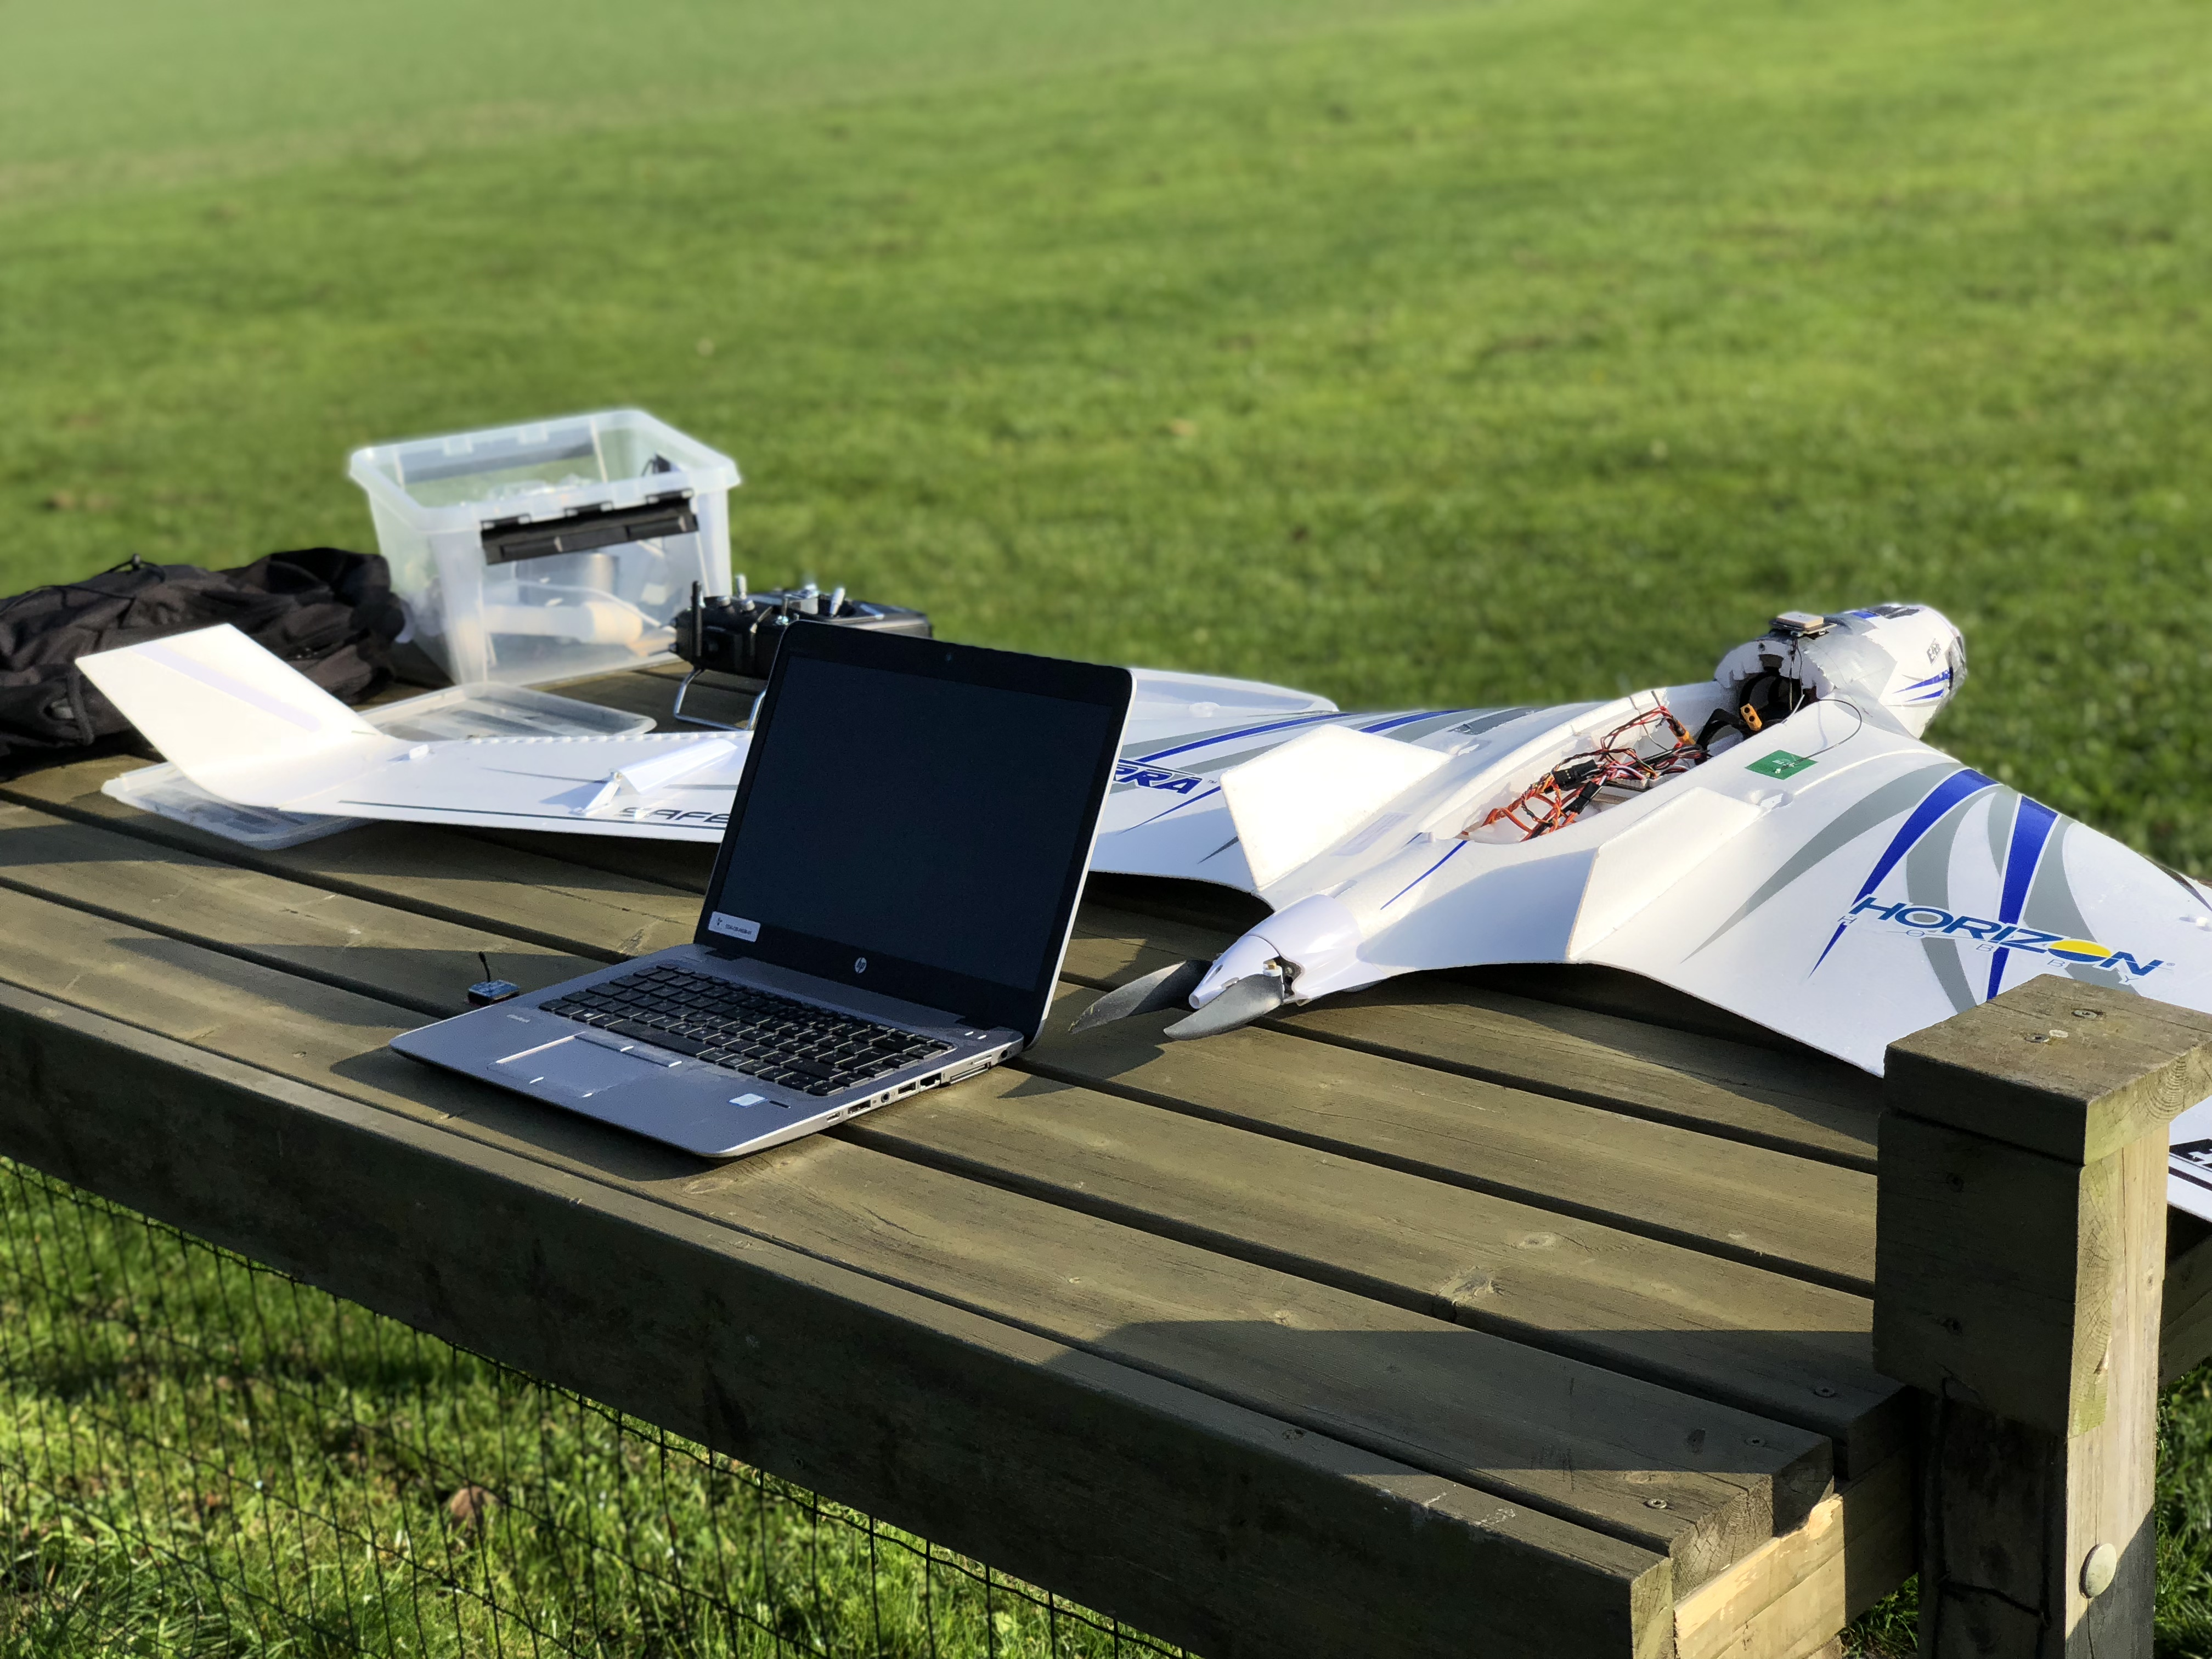
\includegraphics[width=.7\textwidth]{pictures/photo}
  \caption[Opterra fixed-wing drone]{Opterra fixed-wing drone employed as an aerial robotics platform for precision agriculture {\scriptsize(photo credit: Amit Ferencz Appel)}.}   
  \label{fig:opterra}
\end{figure}

We investigate different physical mobile robotics platforms in this work but we focus most on the Opterra fixed-wing drone\findex{Opterra fixed-wing drone}~\citep{opterra} adapted for precision agriculture. Precision agriculture\findex{precision agriculture} is often put into practice~\citep{hajjaj2014review} with ground mobile robots used for harvesting~\citep{qingchun2012study,dong2011development, de2011design, aljanobi2010setup, li2008analysis, edan2000robotic}, and \Gls{acr:uav}s for preventing damage and ensuring better crop quality~\citep{puri2017agriculture, daponte2019review}. The aerial robot is shown in \fref{fig:opterra}{Figure}.

In the remainder of the chapter and before we introduce the problem in \fref{sec:pb-form}{Section}, we briefly investigate the evolution of the field of aerial robotics in the next section. We then analyze the main aerial robots available today, and how they apply to dynamic energy planning in \fref{sec:aerial-robo-types}{Section}. We then provide some further motivation for such planning in \fref{sec:motivation}{Section} and an outline of the approach in \fref{sec:outline}{Section}. Finally, we provide the structure of the remaining chapters in \fref{sec:structure}{Section}.

\section{From UAVs to Modern Aerial Robots}

Modern aerial robots are a valuable tool in robotic research and aerospace. They can be found with different names in the literature. These include unmanned aerial vehicles\findex{unmanned aerial vehicles} (\Gls{acr:uav}s)\footnote{The term unmanned is sometimes replaced by uninhabited if the vehicle is operated remotely by human operator}%citation to Anderson
, unmanned aerial systems\findex{unmanned aerial systems} (\Gls{acr:uas}s), flying robots, or drones. Usually, we refer to drones, \Gls{acr:uav}s, and \Gls{acr:uas}s when these systems are semi-autonomous, or operated from the ground. \Gls{acr:uas} often denote the entire infrastructure of unmanned flight in the aerospace jargon. Aerial or flying robots, on the other hand, have advanced levels of autonomy~\citep{siciliano2016springer}. Nevertheless, all these systems have basic autonomous features such as position and altitude holding, and leveling. The position holding is usually implemented using global navigation satellite system\findex{global navigation satellite system} (\Gls{acr:gnss}), altitude holding using a barometer\findex{barometer}, and leveling using inertial measurement unit\findex{inertial measurement unit} (\Gls{acr:imu}).

\begin{figure}[t]
  \centering
  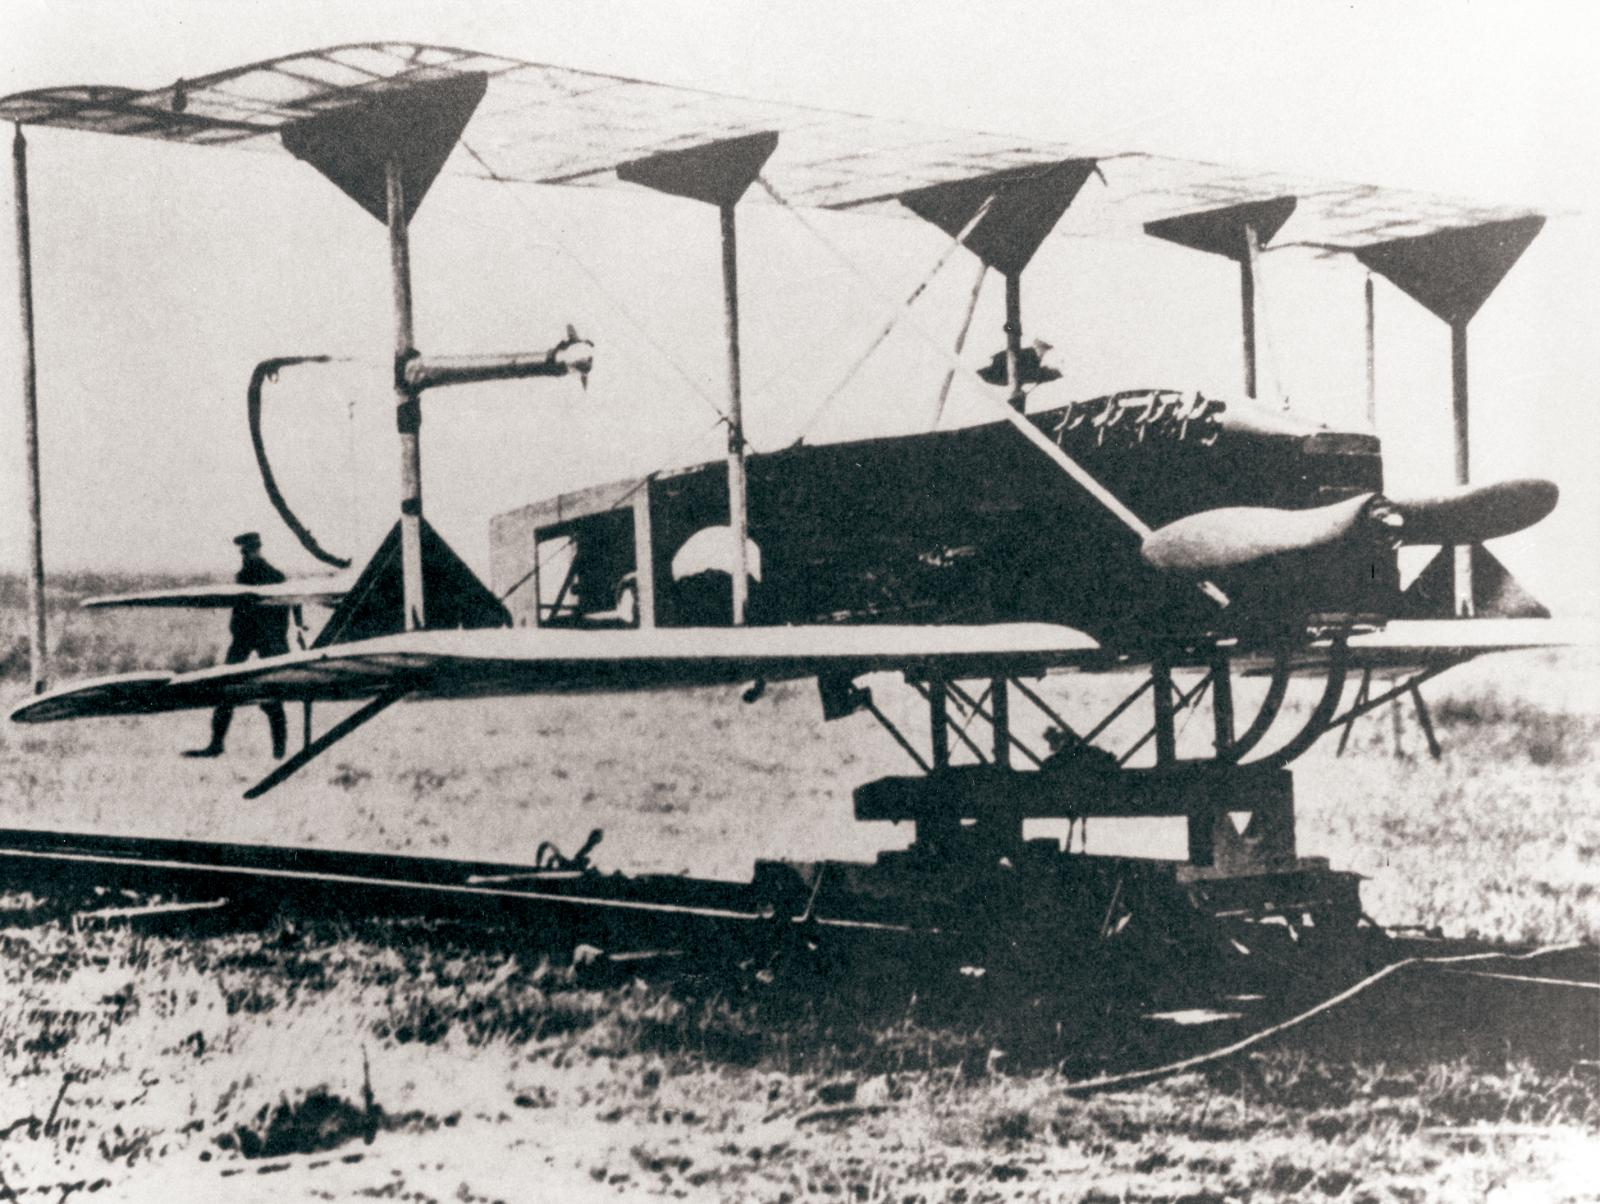
\includegraphics[width=.7\textwidth]{pictures/HA-NH-JA-19_1}
  \caption[Hewitt-Sperry Automatic Airplane, first unmanned flying machine]{The Hewitt-Sperry Automatic Airplane also denominated ``flying bomb'' was developed in WWI and represents the first instance of a \Gls{acr:uav} {\scriptsize(photo credit: United States Naval Institute)}.}   
  \label{fig:hewitt-sperry}
\end{figure}

Uninhabited or unmanned flight has more than a century of developments~\citep{siciliano2016springer}. The origin of the field of aerial robotics, which deals with the design and development of aerial robots, dates back to the first guided missiles~\citep{siciliano2016springer}. Hewitt-Sperry Automatic Airplane\findex{Hewitt-Sperry automatic airplane} developed in 1917 during World War I\findex{World War I} (WWI)~\citep{keane2013brief,valavanis2015handbook} is often referred to as the first unmanned flying machine; a milestone reached relatively soon if we consider that the first heavier-than-air flight in history was demonstrated 14 years earlier with the Wright Flyer I by Wilbur and Orville Wright\findex{Wright brother} (or the Wright brothers). The Hewitt-Sperry Automatic Airplane used a gyroscope\findex{gyroscope}, invented by Elmer Sperry~\citep{keane2013brief}, mechanically connected to the control surfaces and thus successfully integrating a control feedback loop~\citep{siciliano2016springer}. It is shown in \fref{fig:hewitt-sperry}{Figure}.

In the early days, these flying machines were labeled remotely piloted vehicles\findex{remotely piloted vehicles} (\Gls{acr:rpv}s)~\citep{anderson2005introduction}. Many instances from WWI on of such early \Gls{acr:uav}s were designed for military purposes. In the 1950s, United States used a remotely controlled vehicle Ryan Firebee~\findex{Ryan Firebee} for reconnaissance in Vietnam, and Israel used first a \Gls{acr:rpv} in a combat situation~\citep{anderson2005introduction}. Other instances of these vehicles include the V-1 flying bomb~\findex{V-1 flying bomb} from 1944 (deployed by the unified armed forces of nazi Germany) and the Lockheed D-21~\findex{Lockheed D-21} from 1962 (deployed by the United States Air Force).

Global positioning system\findex{global positioning system} (\Gls{acr:gps}) at the end of 1970 opened the possibility for using the \Gls{acr:uav}s for autonomous surveillance, and later integrate them with cameras~\citep{siciliano2016springer}, paving the introduction of modern \Gls{acr:uav}s.

In recent years unmanned flight has been applied in many civilian applications~\citep{gonzalez2017unmanned}. Modern aerial robots are increasingly used in remote sensing\findex{remote sensing}~\citep{noor2018remote,tang2015drone,milas2018drones}, surveillance\findex{surveillance}~\citep{paucar2018use,burkle2009collaborating}, meteorology\findex{meteorology}~\citep{schuyler2019using}, search and rescue\findex{search and rescue}~\citep{pensieri2020drones,karaca2018potential,cui2015drones,seguin2018unmanned}, precision agriculture~\citep{daponte2019review,puri2017agriculture}, transportation, and payload delivery\findex{payload delivery}~\citep{kellermann2020drones}. Although the former four categories do not need advanced autonomy and they fall into the area of reconnaissance, surveillance, and target acquisition\findex{reconnaissance, surveillance, and target acquisition} (\Gls{acr:rsta}), agriculture, transportation, and payload delivery are often realized using to a greater or lesser extent some advanced levels of computational intelligence~\citep{siciliano2016springer}. 

Modern aerial robots are designed to handle unexplored terrain with little interaction as opposed to past \Gls{acr:uav}s operated mainly by a human operator~\citep{siciliano2016springer}. Instances of these systems are in fact expected to autonomously adapt and possibly interact in a broad variety of environmental conditions. 

We conclude this section with a quote from~\citep{anderson2005introduction}: ``the Wright brothers worked so hard to put humans in the air in flying machines, a hundred years later some [...] are working hard to take them out of flying machines''.


\section{Common Classes of Aerial Robots}
\label{sec:aerial-robo-types}

Numerous different types of aerial robots have emerged ever since their first introduction. We briefly investigate the most studied classes in the robotics literature and relate them to the dynamic energy planning that we focus on in this work. 

The two most generic classes are heavier-than-air and lighter-than-air aerial robots.

Heavier-than-air aerial robots\findex{heavier-than-air aerial robots} are divided into fixed- and rotary-wings~\citep{siciliano2016springer}. Some recent developments in bio-inspired robotics study flapping-wings~\citep{floreano2015science}\findex{flapping-wings}. We discuss in detail heavier-than-air aerial robots in this work, as they are a common platform for robotics research. 

Rotary-wing aerial robots\findex{rotary-wings} are highly maneuverable and can perform stationary vertical flight (commonly referred to as hovering\findex{hovering})~\citep{siciliano2016springer}. These systems can be classified into further categories, which include multirotors\findex{multirotors} (such as quadrotors\findex{quadrotors} or quadcopters\findex{quadcopters}, hexacopters\findex{hexacopters}, and octocopters\findex{octocopters}), conventional helicopters\findex{helicopters} (these have one main and one tail rotor), and a coax\findex{coax} (these have counter-rotating coaxial rotors)~\citep{corke2017robotics}.

Fixed-wing aerial robots\findex{fixed-wings} have wings to provide the lift, some control surfaces for maneuvering, and a propeller for forwarding thrust; a shared principle with a common passenger aircraft~\citep{corke2017robotics}. An example constitutes the Opterra adapted for precision agriculture in \fref{fig:opterra}{Figure}.

We discuss the dynamic forces which govern the flight of rotary and fixed-wing aerial robots in \fref{cp:gd}{Chapter}.

Common instances of lighter-than-air aerial robots\findex{lighter-than-air aerial robots} are blimps\findex{blimps} (or non-rigid airships). They usually rely on a gas--such as helium enclosed in a protected envelope~\citep{burri2013design}--to generate the lifting force~\citep{fui2017recent}. An omnidirectional spherical blimp is shown in \fref{fig:skye-blimp}{Figure}. Blimps are similar to balloons but provide basic maneuverability, whereas, in a balloon, only the altitude can be controlled~\citep{colombatti2011lighter}.

\begin{figure}[h]
  \centering
  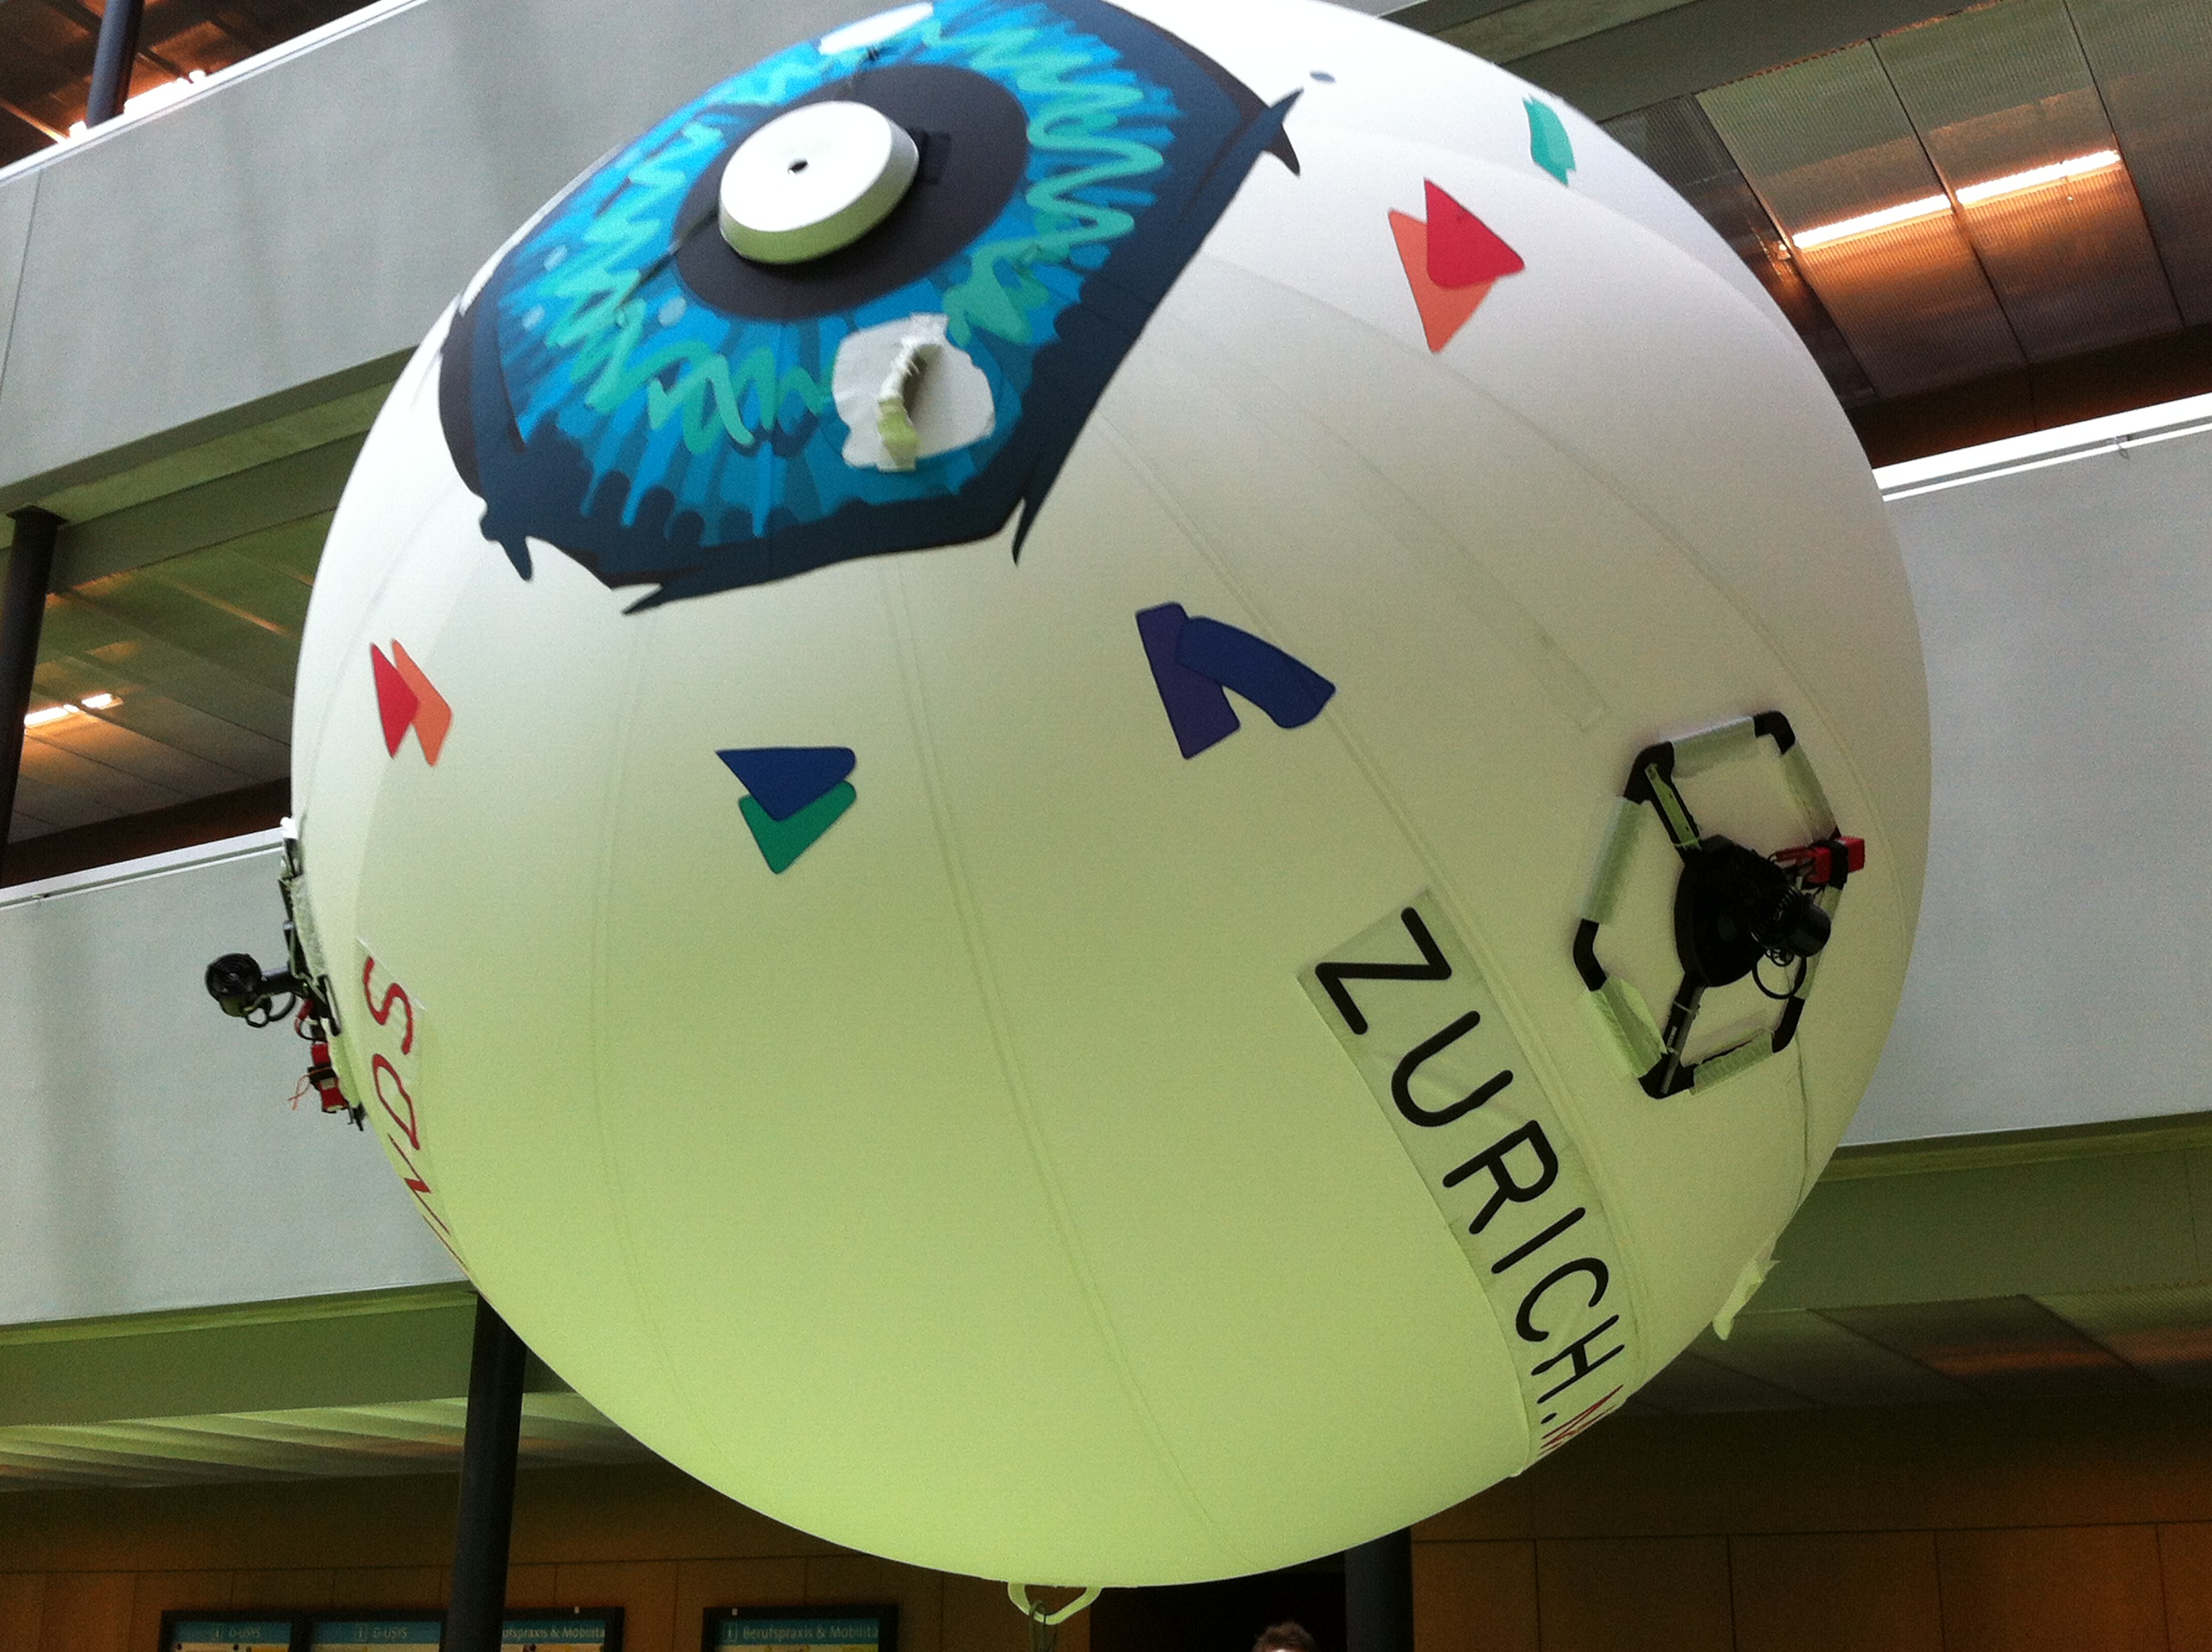
\includegraphics[width=.7\textwidth]{pictures/IMG_2612}
  \caption[Skye, an omnidirectional spherical blimp]{Skye, an omnidirectional spherical blimp developed by ETH Z\"urich. Developed for entertainment purposes, it has a camera system and combines the energy-efficient flight of a blimp with the characteristics of a quadrotor {\scriptsize(photo credit: ETH Z\"urich)}.}   
  \label{fig:skye-blimp}
\end{figure}

Some other classifications found in aerial robotics literature often rely on size and maneuverability and include micro aerial vehicles (MAVs)\findex{micro aerial vehicles}. These are aerial robots with all dimensions lower than 15 cm. Vertical take-off and landing (VTOLs)\findex{vertical take-off and landing} are aerial robots flying in a fixed-wing configuration except if taking-off and landing where they use thrust from rotors rather than lift from wings. 

While rotary-wings are the most maneuverable, less-than-air aerial robots are the least. These, however, have the highest endurance followed by fixed-wing aerial robots. Flapping-wings and mixed configurations, such as VTOLs, fall into the intersection of rotary and fixed-wings for what concerns maneuverability and endurance~\citep{siciliano2016springer}. The energy requirements are critical for all aerial robots, but the difference of motion and computation energy (\Gls{acr:mace}) varies greatly. The energy--inversely proportional to endurance--is highest in rotary-wings and lowest in lighten-than-air aerial robots. The dynamic energy planning approach thus relies on both power-saving task scheduling and energy-efficient path planning for the fixed-wings robots while relying almost exclusively on energy-efficient path planning for rotary-wing aerial robots. In the former \Gls{acr:mace} is close to zero, in the latter is usually high except in energy optimized designs such as some rotary-wing MAVs. Hypothetically, in lighter-than-air aerial robots, \Gls{acr:mace} might be negative; the energy planning approach would rely heavily on power-saving task scheduling.


\section{Motivation}
\label{sec:motivation}

Many applications that involve mobile robots have strict battery limitations. Although this is a common problem to almost any mobile robot, aerial robots are particularly affected. To overcome physical limitations they generally would have to land to recharge or replace the battery~\citep{zamanakos2020energy}. The autonomy of these systems is consequently affected by the availability of the power source. 

A typical example of an aerial robotics scenario in this situation is a robot following a path and performing some onboard computational tasks. For instance, the robot might detect ground patterns and notify other ground-based actors with little human interaction in precision agriculture or another autonomous scenario.

A further complication in these scenarios is that autonomous mobile robots usually carry energy-demanding heterogeneous computing hardware\findex{heterogeneous computing hardware} along a microcontroller\findex{microcontroller} used for basic motion. Computing hardware is involved in path planning and enables autonomous functions, opposed to the microcontroller. The latter runs motion primitives by directly interfacing actuators (such as servos\findex{servo} for the control surfaces\findex{control surface} and motors\findex{motor} for the thrust\findex{thrust} of a fixed-wing aerial robot). The former runs often computer vision and other complex algorithms.

For certain classes of aerial robots with \Gls{acr:mace} close or lower than zero, the autonomy can directly influence the battery state. It is, however, uncommon to find a ready-to-use solution for planning both the path and scheduling the computations of these systems in an energy-aware fashion (we discuss in detail the state-of-the-art in this regard in \fref{cp:soa}{Chapter}). Planning these two aspects simultaneously would pose an advantage in terms of autonomy by optimizing both the path and computations in the function of the battery state of charge (\Gls{acr:soc}). 

Moreover, it is often desirable to reschedule the computations in an energy-aware fashion in-flight phases when the energy needed for motion is different from expected. For instance, a fixed-wing aerial robot might be flying headwinds (with the wind vector parallel and opposite to the direction of motion) and utilizing more energy than planned. It would be of advantage to reschedule the tasks accordingly to save energy needed for motion. During the same flight, the wind direction might suddenly change. The fixed-wing craft, now flying tailwinds, utilizes less energy. It could then potentially increase the level of computations by rescheduling the tasks. In the same flight, the battery might be subject to sudden drops (due to e.g., temperature changes) requiring again replanning by, for instance, shortening the path. It is clear that planning the path and scheduling the computations simultaneously in this scenario is the most desirable course of action.

\subsection{Motion and computation energy}

In the remainder of this work, we refer to computational tasks that can be scheduled in an energy-aware fashion as \emph{computations}, opposed to the other tasks that have no significant effect on energy consumption.

\begin{highlight}
  \begin{defn}[Computations]
    Computations are computational tasks executed on energy-demanding heterogeneous computing hardware carried by a mobile robot along with microcontrollers, sensors, and actuators.
  \end{defn}
\end{highlight}

As an example, we use an aerial robot detecting some patterns while logging the position. Detecting the patterns usually involves heterogeneous computing elements (GPU\findex{GPU} and/or multiple CPU\findex{CPU} cores) and consumes a significant amount of energy as opposed to the log of the position. Detection is a computation, while a log script is (an energy-inexpensive) task.

We refer to the energy that the computations consume as the computation energy, opposed to the motion energy used for physical motion. We use the terms computation and motion energy, and \Gls{acr:mace} several times in the remainder of this work. We thus define these terms formally.

\begin{highlight}
\begin{defn}[Computation/motion energy, \Gls{acr:mace}]
  Given a schedule composed of $i$ computations $s:=\{s_1,s_2,\dots,s_i\}$, the computation energy $E_s(s)$ is the energy spent by heterogeneous computing hardware while executing $s$.
  
  The motion energy is the remaining $E_m$ energy the mobile robot utilizes for the physical motion, for sensing, and for actuating.
\end{defn}
\end{highlight}

Computation and motion energy is measured in watts if instantaneous or joules if over a given time interval.

\begin{highlight}\findex{difference of motion and computational energy}
  \begin{defn}[Difference of motion and computation energy \Gls{acr:mace}]
    The difference of motion and computation energy (\Gls{acr:mace}) is then $E_s-E_m$.
  \end{defn}
\end{highlight}

\subsection{Objective}

We are interested in the energy optimization of the path and computations under uncertainty (atmospheric interferences) in-flight and refer to it as energy dynamic planning.

Such planning would find optimal tradeoffs\findex{tradeoffs} between the path, computations, and energy requirements. Current generic planning solutions for aerial robots do not plan the path and computations dynamically, nor are they energy-aware. They are often semi-autonomous: the path and computations are static and usually defined using planning software~\citep{daponte2019review}. Instances of the planning software include PX4~\citep{px4} and Paparazzi~\citep{papa} flight controllers. Such a state of practice has prompted us to pursue the presented work in dynamic energy planning for aerial robots which plans both the path and computations autonomously while the aerial robot is flying and its batteries draining. 

In our approach, we combined and generalized some of the past body of knowledge on mobile robot planning problems and addressed the increasing computational demands and their relation to energy consumption, path, and autonomy for the mobile robot planning problem. 

We define formally the robot planning problem after outlining the approach in greater detail in the next section.


\section{Outline of the Approach}
\label{sec:outline}

Unlike most of the past mobile robotics planning literature, the approach that we propose plans the path and computations simultaneously. 

The approach necessitates a user-defined initial plan that is replanned energy-wise using the model for future prediction. In the remainder of this work, we progressively build an algorithm that inputs a user-specified initial plan, estimates the model, evaluates future energy consumption, and eventually replans the parameters. 

The initial plan consists of different stages. At each stage, the mobile robot travels a path and executes some computations. The plan then contains some parameters that allow altering the path and computations along with an energy budget.

The alterations are bounded. There is one path constraint set which bounds the path and multiple computation constraint sets, one per each computation parameter, that bound computations.

To model the path we use multiple mathematical functions $\varphi_1,\varphi_2,\dots$. If the path is expressed in 2D at a fixed altitude $h$, the function $\varphi:\mathbb{R}^2\rightarrow\mathbb{R}$ quantifies the distance of a generic point $\mathbf{p}$ in the 2D space from the path. For instance one can define a path as a line
\begin{equation}
  \varphi(x,y):=ax+by+c,
\end{equation}
where $a,b,c$ are given constants. A generic point $\mathbf{p}:=(x_{\mathbf{p}},y_{\mathbf{p}})$ quantifies the distance on the $z$ axis from $ax+by+c=0$. 

\begin{figure}[t]
  \centering
  
\definecolor{cECECEC}{RGB}{236,236,236}
\definecolor{c989898}{RGB}{152,152,152}


\def \globalscale {1.000000}
\begin{tikzpicture}[y=0.80pt, x=0.80pt, yscale=-.9*\globalscale, xscale=.9*\globalscale, inner sep=0pt, outer sep=0pt]
\path[fill=cECECEC,line join=round,line width=0.160pt] (338.3020,263.8010) -- (381.1050,-0.0001) -- (102.8640,12.1601) -- (58.1440,275.9610) -- (338.3020,263.8010) -- cycle;



\path[draw=c989898,line join=round,line width=0.512pt] (147.6250,213.3720) -- (173.5250,186.3120) -- (132.2780,180.7850);



\path[fill=c989898,line join=round,line width=0.256pt] (163.3290,190.5470) -- (158.3650,192.4980) -- (158.1310,191.9020) -- (163.0950,189.9520) -- (163.3290,190.5470) -- cycle(153.4020,194.4490) -- (148.4380,196.4000) -- (148.2040,195.8040) -- (153.1680,193.8530) -- (153.4020,194.4490) -- cycle(143.4740,198.3510) -- (138.5110,200.3020) -- (138.2760,199.7060) -- (143.2400,197.7550) -- (143.4740,198.3510) -- cycle(133.5470,202.2530) -- (128.5830,204.2040) -- (128.3490,203.6080) -- (133.3130,201.6570) -- (133.5470,202.2530) -- cycle(123.6200,206.1550) -- (118.6560,208.1060) -- (118.4220,207.5100) -- (123.3850,205.5590) -- (123.6200,206.1550) -- cycle(113.6920,210.0560) -- (108.7280,212.0070) -- (108.4940,211.4120) -- (113.4580,209.4610) -- (113.6920,210.0560) -- cycle(103.7650,213.9580) -- (100.0090,215.4350) -- (99.7748,214.8390) -- (103.5310,213.3630) -- (103.7650,213.9580) -- cycle(173.2570,186.6450) -- (168.2930,188.5960) -- (168.0590,188.0010) -- (173.0220,186.0500) -- (173.2570,186.6450) -- cycle;



\path[draw=c989898,line join=round,line width=0.512pt] (55.1846,208.3180) -- (99.4269,215.2590);



\path[draw=black,line join=round,line width=0.512pt] (68.2145,216.7950) -- (99.1080,215.5400);



\path[draw=c989898,line join=round,line width=0.512pt] (99.5793,215.0880) -- (196.7320,112.9950);



\path[draw=foo,line join=round,line width=0.512pt] (139.9040,221.4650) -- (147.6230,213.4870);



\path[draw=black,line join=round,line width=0.512pt] (99.6097,215.3190) -- (377.1250,258.8550);



\path[fill=foo,line join=round,line width=0.256pt] (163.7520,67.1159) -- (158.7880,69.0661) -- (158.5540,68.4704) -- (163.5180,66.5202) -- (163.7520,67.1159) -- cycle(153.8240,71.0164) -- (148.8600,72.9667) -- (148.6260,72.3709) -- (153.5900,70.4207) -- (153.8240,71.0164) -- cycle(143.8960,74.9168) -- (138.9320,76.8670) -- (138.6980,76.2713) -- (143.6620,74.3211) -- (143.8960,74.9168) -- cycle(133.9680,78.8173) -- (129.0040,80.7676) -- (128.7700,80.1719) -- (133.7340,78.2216) -- (133.9680,78.8173) -- cycle(124.0400,82.7178) -- (119.0760,84.6679) -- (118.8420,84.0722) -- (123.8060,82.1220) -- (124.0400,82.7178) -- cycle(114.1120,86.6182) -- (109.1480,88.5685) -- (108.9140,87.9728) -- (113.8780,86.0225) -- (114.1120,86.6182) -- cycle(104.1840,90.5187) -- (99.9651,92.1761) -- (99.7311,91.5804) -- (103.9500,89.9230) -- (104.1840,90.5187) -- cycle(173.6800,63.2155) -- (168.7160,65.1657) -- (168.4820,64.5700) -- (173.4460,62.6198) -- (173.6800,63.2155) -- cycle;



\path[draw=black,line join=round,line width=0.512pt] (99.6194,255.8350) -- (99.6701,45.2765);



\path[fill=black,line join=round,line width=0.160pt] (97.4234,50.0749) -- (99.6963,48.0699) -- (101.7800,50.0657) -- (99.5939,44.2973) -- (97.4234,50.0749) -- cycle;



\path[fill=black,line join=round,line width=0.160pt] (372.7840,255.6340) -- (374.2970,258.2610) -- (371.9260,259.9050) -- (378.0140,258.9110) -- (372.7840,255.6340) -- cycle;



\path[draw=c989898,fill=c989898,line join=round,line width=0.160pt] (191.9960,115.1180) -- (195.0250,115.0410) -- (195.3410,117.9090) -- (197.3700,112.0830) -- (191.9960,115.1180) -- cycle;



\path[draw=black,line join=round,line width=0.512pt] (99.6614,215.4240) -- (348.2110,205.3130);



\path[fill=black,line join=round,line width=0.256pt] (365.8960,204.3560) -- (371.2240,204.1220) -- (371.2520,204.7610) -- (365.9240,204.9950) -- (365.8960,204.3560) -- cycle(376.5520,203.8870) -- (381.8800,203.6530) -- (381.9080,204.2920) -- (376.5800,204.5270) -- (376.5520,203.8870) -- cycle(387.2080,203.4190) -- (391.6130,203.2250) -- (391.6410,203.8640) -- (387.2370,204.0580) -- (387.2080,203.4190) -- cycle(355.2390,204.8250) -- (360.5670,204.5900) -- (360.5960,205.2300) -- (355.2670,205.4640) -- (355.2390,204.8250) -- cycle;



\path[fill=black,line join=round,line width=0.256pt] (51.6916,217.8380) -- (46.3616,218.0290) -- (46.3388,217.3890) -- (51.6687,217.1990) -- (51.6916,217.8380) -- cycle(41.0317,218.2190) -- (35.7017,218.4090) -- (35.6789,217.7700) -- (41.0088,217.5790) -- (41.0317,218.2190) -- cycle(30.3718,218.6000) -- (25.0419,218.7900) -- (25.0190,218.1500) -- (30.3490,217.9600) -- (30.3718,218.6000) -- cycle(62.3514,217.4570) -- (57.0215,217.6480) -- (56.9986,217.0080) -- (62.3286,216.8180) -- (62.3514,217.4570) -- cycle;



\path[draw=black,line join=round,line width=0.512pt] (138.1150,223.3150) -- (140.0590,221.3710);



\path[draw=c989898,line join=round,line width=0.512pt] (129.6630,180.5070) -- (132.3930,180.8300);



\path[draw=c989898,line join=round,line width=0.512pt] (173.5260,186.3500) -- (173.5730,63.0377);



\path[draw=black,line join=round,line width=0.512pt] (96.7492,91.8181) -- (99.4988,91.8249);



\path[cm={{1.0,0.0,0.0,1.0,(376.0,276.0)}}] (0.0000,0.0000) node[above right] () {$x$};



\path[cm={{1.0,0.0,0.0,1.0,(198.0,102.0)}}] (0.0000,0.0000) node[above right] () {$y$};



\path[cm={{1.0,0.0,0.0,1.0,(85.0,46.0)}}] (0.0000,0.0000) node[above right] () {$z$};



\path[draw=black,line join=round,line width=0.512pt] (83.3760,232.1090) -- (99.6032,215.0620);



\path[fill=c989898,line join=round,line width=0.512pt] (173.2360,184.7230) .. controls (174.0900,184.7230) and (174.7820,185.4150) .. (174.7820,186.2700) .. controls (174.7820,187.1240) and (174.0900,187.8160) .. (173.2360,187.8160) .. controls (172.3810,187.8160) and (171.6890,187.1240) .. (171.6890,186.2700) .. controls (171.6890,185.4150) and (172.3810,184.7230) .. (173.2360,184.7230) -- cycle;



\path[cm={{1.0,0.0,0.0,1.0,(161.0,289.0)}}] (0.0000,0.0000) node[above right] () {$\varphi(x,y):=2y-x$};



\path[cm={{1.0,0.0,0.0,1.0,(353.0,224.0)}}] (0.0000,0.0000) node[above right] () {$2y-x=0$};



\path[cm={{1.0,0.0,0.0,1.0,(131.0,238.0)}}] (0.0000,0.0000) node[above right] () {$x_\mathbf{p}$};



\path[cm={{1.0,0.0,0.0,1.0,(113.0,180.9)}}] (0.0000,0.0000) node[above right] () {$y_\mathbf{p}$};



\path[cm={{1.0,0.0,0.0,1.0,(41.0,98.0)}}] (0.0000,0.0000) node[above right] () {$\varphi(\mathbf{p})=d$};



\path[draw=c989898,fill=c989898,line join=round,line width=0.160pt] (175.7670,179.7880) -- (173.4940,181.7930) -- (171.4110,179.7970) -- (173.5970,185.5660) -- (175.7670,179.7880) -- cycle;



\path[draw=c989898,fill=c989898,line join=round,line width=0.160pt] (171.2840,70.1412) -- (173.5570,68.1363) -- (175.6400,70.1321) -- (173.4540,64.3637) -- (171.2840,70.1412) -- cycle;



\path[fill=foo,line join=round,line width=0.512pt] (173.4160,61.7418) .. controls (174.2700,61.7418) and (174.9630,62.4342) .. (174.9630,63.2885) .. controls (174.9630,64.1427) and (174.2700,64.8351) .. (173.4160,64.8351) .. controls (172.5620,64.8351) and (171.8700,64.1427) .. (171.8700,63.2885) .. controls (171.8700,62.4342) and (172.5620,61.7418) .. (173.4160,61.7418) -- cycle;



  \path[fill=cECECEC,line join=round,line width=0.160pt] (182.5940,102.1690) -- (164.2430,102.1690) -- (164.1940,119.9680) -- (182.5870,119.9220) -- (182.5940,102.1690) -- cycle;



  \path[cm={{1.0,0.0,0.0,1.0,(170.0,116.0)}}] (0.0000,0.0000) node[above right] () {$d$};



\path[cm={{1.0,0.0,0.0,1.0,(187.0,186.0)}}] (0.0000,0.0000) node[above right] () {$(x_\mathbf{p},y_\mathbf{p},0)$};




\end{tikzpicture}


  \caption[Concept of the path and generic point in space]{If we define the path as mathematical function $\varphi$ at a fixed altitude $h$, a generic point $p$ in 2D space quantifies the distance $d$ on the $z$ axis from $h$.}
  \label{fig:plot1}
\end{figure}

The concept is shown in \fref{fig:plot1}{Figure} for $c$ zero and $a,b$ minus one and two respectively. A generic point $\mathbf{p}:=(x_{\mathbf{p}},y_{\mathbf{p}})$ intersects the plane
\begin{equation}
  \varphi(x,y):=2y-x,
\end{equation}
at $z=\varphi(\mathbf{p})$. The path at a fixed altitude is then $\varphi(x,y)=0$, or more generally $\varphi(x,y)=h$ with $h\in\mathbb{R}$.

We use this concept to model complex paths. For instance, the path might contain multiple circles and lines{\color{red}, as shown in \dots. The aerial robot travels the path using vector field for guidance (we describe in detail such vector field in \fref{cp:gd}{Chapter}) and switches between the trajectories as soon as it reaches specific triggering points}. 

To model the computations we use \powprof{}, a profiling tool presented in~\citep{seewald2019coarse}. To guide the UAV we use a vector field~\citep{de2017guidance} that converges to the path. The use of vector fields for guidance is widely discussed in the literature~\citep{lindemann2005smoothly,gonccalves2010vector,panagou2014motion,zhou2014vector,kapitanyuk2017guiding,de2017guidance}. 

To achieve the energy-aware dynamic planning, we further introduce and formally prove a periodic energy model that accounts for the uncertainty. We use Fourier analysis to derive the model, and state estimation to address the uncertainty. Periodicity is often present due to repetitive patterns in the plan~\citep{seewald2020mechanical}. Indeed, mobile robots often iterate over a set of tasks and paths. Given that the plan is periodic, we expect the energy consumption to approximately evolve periodically. We describe in detail such model in \fref{cp:model}{Chapter}. 

Some collected energy data from the Opterra (\fref{fig:opterra}{Figure}) adapted for precision agriculture along its power spectrum motivates our choice {\color{red}in \dots \fref{}{Figure} and \dots}. 

We replan the path and computations with model predictive control (MPC)~\cite{rawlings2017model}. The control is data-driven. Energy sensor data estimates some coefficients of an energy model used to predict future energy consumption in presence of uncertainty. The energy budget is the battery capacity and other battery parameters. These are fixed values that are not replanned by the algorithm. Our goal is to complete the plan with the highest possible parameters configuration as the mobile robot executes the plan and its batteries drain. 

\subsection{Applications}

The dynamic energy planning in this work applies mostly to modern aerial robots with a certain degree of autonomy in the sense that the aerial robot is assumed to perform a predefined set of tasks over a given space. Although most of the guidance in \fref{cp:gd}{Chapter} is specifically meant for aerial robots, the approach can be easily adapted to other energy-constrained mobile robots. For instance, we have applied the approach to the space robotics context~\citep{seewald2020beyond}. We discuss this further in \fref{cp:conc}{Chapter}.

We specifically focus and show the performance on a search and rescue and precision agriculture scenario implemented with aerial robots. In fact, precision agriculture is often put into practice~\citep{hajjaj2014review} with ground mobile robots used for harvesting~\citep{qingchun2012study,dong2011development, de2011design, aljanobi2010setup, li2008analysis, edan2000robotic}, and aerial robots for preventing damage and ensuring better crop quality~\citep{puri2017agriculture, daponte2019review}. 

In the search and rescue scenario, the aerial robot performs autonomous detections of patterns over the sea. In this scenario, we mostly focus on the validation of the computation energy model (described in detail in \fref{}{}).

In the precision agriculture scenario, the aerial robot covers a given agricultural field (a polygon) and search for ground hazards. The plan is structured as follows. Path-wise, the Opterra fixed-wing drone from \fref{fig:opterra}{Figure} flies in circles and lines covering the polygon. Computation-wise, it detects hazards using a neural network and notifies grounded mobile robots employed for, e.g., harvesting. The approach alters the plan; it controls the processing rate and the radius of the circles affecting the distance between the lines. 

We observe that not only the path but also the computations significantly impact the energy, with a potential extension of up to 13 minutes over an hour by switching from the highest to the lowest level of computations in presence of a standard battery.

\section{Problem Formulation}
\label{sec:pb-form}

To formulate the mobile robot planning problem we adopt to the following mathematical notation. We apply later the formulation to both the search and rescue and the precision agriculture scenario.

Given an integer $x\in\mathbb{Z}_{\geq 0}$, we use the notation $[x]$ for the set $\{0,1,\dots,x\}\subseteq\mathbb{Z}_{\geq 0}$. The notation $[x]_{>0}$ for the set $\{1,2,\dots,x\}\subseteq\mathbb{Z}_{> 0}$ or simply $[x]/\{0\}$ with $x\in\mathbb{Z}_{>0}$. We use bold lower-case letters $\mathbb{x}$ for the vectors.

We use extensively the term parameters. These are variable values that we use to dynamically plan path and computations. $c_{i,j}$ denotes the $j$-th parameter of the $i$-th parameters set $c_i$. $\underline{c}_{i,j}$ is the lower bound of the parameter $c_{i,j}$. $\overline{c}_{i,j}$ is the upper bound of the parameter $c_{i,j}$, i.e., $\underline{c}_{i,j}\leq c_{i,j}\leq\overline{c}_{i,j}$.

Let us assume that the path at stage $i$ can be altered with $\rho$ path parameters
\begin{equation}\label{eq:path-params}
    c_i^\rho:=\{c_{i,1},c_{i,2},\dots,c_{i,\rho}\},
\end{equation}
and the computations with $\sigma$ computation parameters 
\begin{equation}\label{eq:comp-params}
    c_i^\sigma:=\{c_{i,\rho+1},c_{i,\rho+2},\dots,c_{i,\rho+\sigma}\}.
\end{equation}

We then express the path as a continuous twice differentiable function $\varphi_i:\mathbb{R}^2\times\mathbb{R}^\rho\rightarrow\mathbb{R}$ of a point and the path parameters. The function returns a metric of the distance between the point and the nominal trajectory. We express the computations as the value of the computation parameters. We discuss the concrete meaning of the value of path parameters in \fref{cp:model}{Chapter}.

\begin{highlight}  
  \begin{defn}[Stage]\label{def:mission}
    The $i$-th \emph{stage} $\Gamma_i$ at time instant $t$ of a plan $\Gamma$ is
    \begin{equation*}\begin{split}
      \Gamma_i:=\{\varphi_i(\mathbf{p}(t),c_i^\rho),c_i^\sigma\mid
      \,&\exists\,\,\mathbf{p}(t),\,\varphi_i(\mathbf{p}(t),c_i^\rho)\in\mathcal{C}_i,\,\\
        &\,\forall j\in[\sigma]^+,\,c_{i,\rho+j}\in\mathcal{S}_{i,j}\,\},
    \end{split}\end{equation*}
    where $\mathcal{C}_i:=[\underline{c}_i,\overline{c}_i]\subseteq\mathbb{R}$ is the path constraint set, and $\mathcal{S}_{i,j}:=[\underline{c}_{i,\rho+j},\overline{c}_{i,\rho+j}]\subseteq\mathbb{Z}_{\geq 0}$ the $j$-th computation constraint set. 
    
    $\mathbf{p}(t)$ is a point of a mobile robot travelling at an altitude $h\in\mathbb{R}_{\geq 0}$ with respect to some inertial navigation frame $\mathcal{O}_W$.
  \end{defn}
\end{highlight}

\begin{highlight}  
  \begin{defn}[Plan]
    The \emph{plan} is a finite state machine (FSM) $\Gamma$ where the state-transition function $s:\bigcup_i{\Gamma_i}\times\mathbb{R}^2\rightarrow\bigcup_i{\Gamma_i}$ maps a stage and a point to the next stage
    \begin{equation*}s(\Gamma_i,\mathbf{p}_k):=\begin{cases}
      \Gamma_{i+1} & \text{if }\mathbf{p}_k=\mathbf{p}_{\Gamma_i}\\
      \Gamma_i & \text{otherwise}
    \end{cases}.\end{equation*}
  \end{defn}
\end{highlight}

\begin{highlight}  
  \begin{defn}[Triggering, and final point]\label{def:mission}
    The point $\mathbf{p}_{\Gamma_{i}}$ that allows the transition between $\Gamma_i$ and $\Gamma_{i+1}$ is called \emph{triggering point}. The last triggering point $\mathbf{p}_{\Gamma_{l}}$ relative to the last stage $\Gamma_l$ is called \emph{final point}.
  \end{defn}
\end{highlight}

\begin{figure}[h]
  \center
  \begin{tikzpicture}[shorten >=.5pt,node distance=12.5ex,on grid,auto,initial text=\footnotesize\fontfamily{phv}\selectfont{start}]
    \node[state,initial] (q_i) {$\Gamma_1$}; 
    \node        [right=of q_i] (q_dots0) {$\cdots$};
    \node[state] (q_0) [right=of q_dots0] {$\Gamma_i$};
    \node        (q_dots1) [right=of q_0] {$\cdots$};
    \node[state,accepting] (q_f) [right=of q_dots1] {$\Gamma_f$};
    \path[->]
    (q_i) edge node {$\mathbf{p}_{\Gamma_{1}}$} (q_dots0)
    (q_dots0) edge node{$\mathbf{p}_{\Gamma_{i-1}}$} (q_0)
    (q_0) edge node {$\mathbf{p}_{\Gamma_i}$} (q_dots1)
    (q_dots1) edge node {$\mathbf{p}_{\Gamma_{l}}$} (q_f)    
    (q_i) edge [loop above] node {$\mathbf{p}_{k_1}$} (q_i)
    (q_0) edge [loop above] node {$\mathbf{p}_{k_2}$} (q_0)
    (q_f) edge [loop above] node {$\mathbf{p}_{k_3}$} (q_f)
    ; %end path 
    \draw [decorate,decoration={brace,amplitude=10pt,mirror,raise=10pt},yshift=0pt]
    (q_i.south west) -- (q_f.south west) node [black,midway,yshift=-9ex]{$\Gamma$};
  \end{tikzpicture}
  \caption{The plan defined as a FSM}
  \label{fig:state-machine}
\end{figure}

\begin{figure}[t]
    \centering
    
\definecolor{c989898}{RGB}{152,152,152}
\definecolor{cDEDEDE}{RGB}{222,222,222}
\definecolor{cFFFFFF}{RGB}{255,255,255}
\definecolor{c2B2B2B}{RGB}{43,43,43}
\definecolor{c9B9B9B}{RGB}{155,155,155}


\def \globalscale {1.000000}
\begin{tikzpicture}[y=0.80pt, x=0.80pt, yscale=-1.1*\globalscale, xscale=1.1*\globalscale, inner sep=0pt, outer sep=0pt]
\path[draw=c989898,line join=round,line width=0.512pt] (37.9773,138.5660) -- (35.3357,138.5630);



  \path[fill=cDEDEDE,line join=round,even odd rule,line width=0.160pt] (59.2379,138.5360) -- (37.3300,138.5360) .. controls (37.3300,104.2680) and (65.1100,76.4881) .. (99.3784,76.4881) -- (99.3784,98.1778) .. controls (77.1987,98.3164) and (59.2589,116.3290) .. (59.2379,138.5360) -- cycle;



  \path[fill=cDEDEDE,line join=round,even odd rule,line width=0.160pt] (36.8146,208.2220) -- (59.2401,208.2220) -- (59.2407,138.0860) -- (36.8151,138.0860) -- (36.8146,208.2220) -- cycle;



  \path[fill=cDEDEDE,line join=round,even odd rule,line width=0.160pt] (75.5064,138.3220) -- (53.5984,138.3220) .. controls (53.5984,104.0540) and (81.3785,76.2741) .. (115.6470,76.2741) -- (115.6470,97.9639) .. controls (93.4671,98.1025) and (75.5273,116.1150) .. (75.5064,138.3220) -- cycle;



  \path[fill=cDEDEDE,line join=round,even odd rule,line width=0.160pt] (115.5600,97.9479) -- (115.5600,76.0399) .. controls (149.8280,76.0399) and (177.7080,103.8200) .. (177.7080,138.0880) -- (156.0190,138.0880) .. controls (155.8800,115.9090) and (137.7680,97.9688) .. (115.5600,97.9479) -- cycle;



  \path[fill=cDEDEDE,line join=round,even odd rule,line width=0.160pt] (53.0716,208.2330) -- (75.4972,208.2330) -- (75.4974,138.0950) -- (53.0718,138.0950) -- (53.0716,208.2330) -- cycle;



  \path[fill=cDEDEDE,line join=round,even odd rule,line width=0.160pt] (155.9570,208.2190) -- (178.3830,208.2190) -- (178.3990,137.9630) -- (155.9730,137.9630) -- (155.9570,208.2190) -- cycle;



  \path[draw=c989898,line join=round,line width=0.512pt] (99.5543,138.9930) ellipse (1.7511cm and 1.7511cm);



  \path[cm={{1.0,0.0,0.0,1.0,(190.0,175.0)}}] (0.0000,0.0000) node[above right] () {$\mathbf{p}_{k_4}$};



    \path[fill=cFFFFFF,line join=round,line width=0.160pt,rounded corners=0.0000cm] (65.5184,186.6300) rectangle (81.7257,202.8374);



    \path[cm={{1.0,0.0,0.0,1.0,(66.0,199.0)}}] (0.0000,0.0000) node[above right] () {$\varphi_1$};



  \path[draw=c2B2B2B,line join=round,line width=0.512pt] (115.6970,138.4880) ellipse (1.7511cm and 1.7511cm);



  \path[draw=c2B2B2B,line join=round,line width=0.512pt] (53.2806,50.4116) -- (53.2808,208.0220);



  \path[draw=c2B2B2B,line join=round,line width=0.512pt] (177.8300,50.4301) -- (177.8300,208.0410);



  \path[draw=c2B2B2B,line join=round,line width=0.512pt] (118.1030,140.8340) -- (113.8230,136.5520);



  \path[draw=c2B2B2B,line join=round,line width=0.512pt] (113.8260,140.8310) -- (118.1070,136.5500);



  \path[fill=black,line join=round,line width=0.256pt] (52.5078,197.6220) -- (52.5078,192.2880) -- (53.7878,192.2880) -- (53.7878,197.6220) -- (52.5078,197.6220) -- cycle(52.5078,186.9550) -- (52.5077,181.6220) -- (53.7877,181.6220) -- (53.7877,186.9550) -- (52.5078,186.9550) -- cycle(52.5077,176.2890) -- (52.5077,170.9550) -- (53.7877,170.9550) -- (53.7877,176.2890) -- (52.5077,176.2890) -- cycle(52.5077,165.6220) -- (52.5077,160.2890) -- (53.7877,160.2890) -- (53.7877,165.6220) -- (52.5077,165.6220) -- cycle(52.5076,154.9550) -- (52.5076,149.6220) -- (53.7876,149.6220) -- (53.7876,154.9550) -- (52.5076,154.9550) -- cycle(52.5076,144.2890) -- (52.5076,138.9550) -- (53.7876,138.9550) -- (53.7876,144.2890) -- (52.5076,144.2890) -- cycle(53.0267,133.5810) -- (53.1252,132.8330) -- (53.8254,128.9130) -- (53.9747,128.2740) -- (55.2289,128.5300) -- (55.0796,129.1680) -- (54.3905,133.0260) -- (54.2992,133.7200) -- (53.0267,133.5810) -- cycle(55.2719,123.0650) -- (56.4670,119.0750) -- (56.8957,117.9440) -- (58.1090,118.3510) -- (57.6804,119.4830) -- (56.5094,123.3920) -- (55.2719,123.0650) -- cycle(58.8505,112.9310) -- (61.1435,108.1160) -- (62.3221,108.6150) -- (60.0291,113.4300) -- (58.8505,112.9310) -- cycle(63.8781,103.4730) -- (64.7913,101.9480) -- (66.9793,99.0624) -- (68.0419,99.7761) -- (65.8539,102.6620) -- (65.0079,104.0740) -- (63.8781,103.4730) -- cycle(70.4287,94.9101) -- (74.1486,91.0881) -- (75.1213,91.9201) -- (71.4014,95.7421) -- (70.4287,94.9101) -- cycle(78.4053,87.7408) -- (80.3745,86.2019) -- (82.9136,84.7517) -- (83.6288,85.8132) -- (81.0897,87.2634) -- (79.2622,88.6916) -- (78.4053,87.7408) -- cycle(87.6306,82.0689) -- (92.6007,80.1345) -- (93.1529,81.2893) -- (88.1827,83.2237) -- (87.6306,82.0689) -- cycle(97.7391,78.4275) -- (102.9360,77.2307) -- (103.3130,78.4540) -- (98.1160,79.6508) -- (97.7391,78.4275) -- cycle(108.2830,76.3988) -- (113.5950,75.9193) -- (113.7960,77.1835) -- (108.4840,77.6630) -- (108.2830,76.3988) -- cycle(119.0310,75.9276) -- (124.3360,76.4738) -- (124.2840,77.7527) -- (118.9790,77.2066) -- (119.0310,75.9276) -- cycle(129.6590,77.4030) -- (134.8450,78.6494) -- (134.6300,79.9113) -- (129.4440,78.6648) -- (129.6590,77.4030) -- cycle(139.9380,80.4796) -- (144.0440,82.1042) -- (144.9200,82.6049) -- (144.3640,83.7578) -- (143.4890,83.2571) -- (139.5520,81.7000) -- (139.9380,80.4796) -- cycle(149.5490,85.2532) -- (150.9890,86.0768) -- (153.9650,88.3831) -- (153.2520,89.4460) -- (150.2750,87.1396) -- (148.9930,86.4062) -- (149.5490,85.2532) -- cycle(158.1060,91.8657) -- (161.8580,95.6554) -- (161.0080,96.6118) -- (157.2550,92.8221) -- (158.1060,91.8657) -- cycle(165.1950,99.9168) -- (166.1480,101.1420) -- (168.1780,104.4180) -- (167.1250,105.1460) -- (165.0960,101.8700) -- (164.2320,100.7590) -- (165.1950,99.9168) -- cycle(170.7940,109.1320) -- (172.2860,112.1330) -- (173.0420,114.0250) -- (171.8730,114.5450) -- (171.1170,112.6530) -- (169.6740,109.7510) -- (170.7940,109.1320) -- cycle(174.9250,119.0630) -- (175.9740,122.3380) -- (176.4510,124.2150) -- (175.2200,124.5650) -- (174.7430,122.6880) -- (173.7200,119.4930) -- (174.9250,119.0630) -- cycle(177.6310,129.4510) -- (177.8280,130.4450) -- (178.2610,133.3030) -- (178.4240,134.7830) -- (177.1550,134.9460) -- (176.9910,133.4660) -- (176.5670,130.6630) -- (176.3820,129.7310) -- (177.6310,129.4510) -- cycle(178.5140,140.1950) -- (178.5100,145.5280) -- (177.2300,145.5270) -- (177.2340,140.1940) -- (178.5140,140.1950) -- cycle(178.5060,150.8610) -- (178.5020,156.1950) -- (177.2220,156.1940) -- (177.2260,150.8600) -- (178.5060,150.8610) -- cycle(178.4970,161.5280) -- (178.4930,166.8610) -- (177.2130,166.8600) -- (177.2170,161.5270) -- (178.4970,161.5280) -- cycle(178.4890,172.1950) -- (178.4850,177.5280) -- (177.2050,177.5270) -- (177.2090,172.1940) -- (178.4890,172.1950) -- cycle(178.4810,182.8610) -- (178.4800,184.3970) -- (177.2000,184.3960) -- (177.2010,182.8600) -- (178.4810,182.8610) -- cycle(52.5078,208.2880) -- (52.5078,202.9550) -- (53.7878,202.9550) -- (53.7878,208.2880) -- (52.5078,208.2880) -- cycle;



    \path[fill=cFFFFFF,line join=round,line width=0.160pt,rounded corners=0.0000cm] (170.4340,62.4618) rectangle (186.6414,78.6691);



    \path[cm={{1.0,0.0,0.0,1.0,(170.0,75.0)}}] (0.0000,0.0000) node[above right] () {$\varphi_4$};



  \path[fill=cFFFFFF,line join=round,line width=0.160pt,rounded corners=0.0000cm] (151.1930,87.1333) rectangle (167.4004,103.3407);



  \path[cm={{1.0,0.0,0.0,1.0,(154.0,98.0)}}] (0.0000,0.0000) node[above right] () {$\varphi_5$};



  \path[cm={{1.0,0.0,0.0,1.0,(16.0,120.0)}}] (0.0000,0.0000) node[above right] () {$\mathbf{p}_{k_3}$};



  \path[draw=c989898,line join=round,line width=0.512pt] (101.6410,140.7130) -- (97.3588,136.4310);



  \path[draw=c989898,line join=round,line width=0.512pt] (97.3620,140.7090) -- (101.6430,136.4300);



  \path[draw=c989898,line join=round,line width=0.512pt] (37.4683,50.2362) -- (37.4674,207.8470);



  \path[draw=black,line join=round,line width=1.024pt] (37.3655,139.1460) .. controls (37.3655,108.3180) and (59.8482,82.7404) .. (89.3117,77.9160);



  \path[draw=black,line join=round,line width=1.024pt] (37.4074,138.8430) -- (37.4612,139.4260);



  \path[draw=black,line join=round,line width=1.024pt] (104.8160,14.6465) .. controls (114.1410,17.1626) and (116.3470,26.7356) .. (116.3470,26.7355) .. controls (116.3470,26.7355) and (134.0140,69.7724) .. (87.7439,78.3357);



  \path[draw=black,fill=cFFFFFF,line join=round,line width=0.512pt] (38.0214,129.9470) -- (48.4265,113.7660) -- (41.6299,114.7590) -- (36.4969,110.7700) -- (38.0214,129.9470) -- cycle;



  \path[draw=black,line join=round,line width=1.024pt] (37.3995,208.3130) -- (37.3999,138.8280);



    \path[fill=cFFFFFF,line join=round,line width=0.160pt,rounded corners=0.0000cm] (48.2360,62.4618) rectangle (64.4433,78.6691);



    \path[cm={{1.0,0.0,0.0,1.0,(46.0,75.0)}}] (0.0000,0.0000) node[above right] () {$\varphi_6$};



  \path[draw=black,line join=round,line width=0.512pt] (38.2486,129.1090) -- (41.5789,114.8440);



  \path[draw=black,fill=cFFFFFF,line join=round,line width=0.512pt] (75.8501,81.3976) -- (95.0620,82.3957) -- (90.0278,77.8124) -- (91.7396,70.5527) -- (75.8501,81.3976) -- cycle;



  \path[draw=black,line join=round,line width=0.512pt] (76.2742,81.2804) -- (89.9006,77.8114);



  \path[draw=black,line join=round,line width=1.024pt] (177.8490,208.2210) -- (177.8490,158.6520);



  \path[draw=black,fill=c9B9B9B,line join=round,line width=0.512pt] (177.8340,156.5720) -- (171.4330,174.7140) -- (177.8190,172.1830) -- (183.7320,174.8830) -- (177.8340,156.5720) -- cycle;



  \path[draw=black,line join=round,line width=0.512pt] (177.8060,157.4410) -- (177.8490,172.0900);



  \path[draw=black,fill=cFFFFFF,line join=round,line width=0.512pt] (122.5820,36.7240) -- (118.0690,18.0488) -- (113.9380,22.8537) -- (107.6780,24.6001) -- (122.5820,36.7240) -- cycle;



  \path[draw=black,line join=round,line width=0.512pt] (11.2790,8.9418) -- (11.2790,38.5413);



  \path[draw=black,line join=round,line width=0.512pt] (40.6757,38.3017) -- (11.0761,38.3017);



  \path[cm={{1.0,0.0,0.0,1.0,(1.0,52.0)}}] (0.0000,0.0000) node[above right] () {$\mathcal{O}_W$};



  \path[draw=black,line join=round,line width=0.512pt] (12.2122,38.1596) -- (114.5840,24.7774);



    \path[fill=cFFFFFF,line join=round,line width=0.160pt,rounded corners=0.0000cm] (49.3746,20.2690) rectangle (73.7139,36.4553);



    \path[cm={{1.0,0.0,0.0,1.0,(53.0,35.0)}}] (0.0000,0.0000) node[above right] () {$\mathbf{p}_{k_1}$};



  \path[draw=black,line join=round,line width=0.512pt] (113.9240,22.8546) -- (122.4610,36.6020);



  \path[fill=black,line join=round,line width=0.160pt] (38.7120,35.2069) -- (38.7201,41.3379) -- (44.3321,38.2655) -- (38.7120,35.2069) -- cycle;



  \path[fill=black,line join=round,line width=0.160pt] (8.2258,10.6325) -- (14.3568,10.6281) -- (11.2877,5.0143) -- (8.2258,10.6325) -- cycle;



  \path[fill=black,line join=round,line width=0.160pt] (109.5870,22.7566) -- (110.5860,28.8056) -- (115.6270,24.8662) -- (109.5870,22.7566) -- cycle;



    \path[fill=cFFFFFF,line join=round,line width=0.160pt,rounded corners=0.0000cm] (29.9808,62.4618) rectangle (46.1881,78.6691);



    \path[cm={{1.0,0.0,0.0,1.0,(27.0,75.0)}}] (0.0000,0.0000) node[above right] () {$\varphi_2$};



\path[draw=c2B2B2B,line join=round,line width=0.512pt] (179.6380,138.6350) -- (177.4990,138.6330);



\path[draw=c2B2B2B,line join=round,line width=0.512pt] (53.7370,138.6060) -- (51.0981,138.6060);



  \path[fill=cFFFFFF,line join=round,line width=0.160pt] (185.5880,202.9890) -- (173.1380,202.9890) -- (173.1040,215.0630) -- (185.5830,215.0320) -- (185.5880,202.9890) -- cycle;



  \path[cm={{1.0,0.0,0.0,1.0,(176.0,213.0)}}] (0.0000,0.0000) node[above right] () {$\overline{c}_4$};



  \path[fill=cFFFFFF,line join=round,line width=0.160pt] (160.5750,202.9910) -- (148.1260,202.9910) -- (148.0920,215.0660) -- (160.5710,215.0350) -- (160.5750,202.9910) -- cycle;



  \path[cm={{1.0,0.0,0.0,1.0,(151.0,213.0)}}] (0.0000,0.0000) node[above right] () {$\underline{c}_4$};




\path[cm={{1.0,0.0,0.0,1.0,(14.0,143.0)}}] (0.0000,0.0000) node[above right] () {$\mathbf{p}_{\Gamma_1}$};



\path[fill=cFFFFFF,line join=round,line width=0.160pt,rounded corners=0.0000cm] (62.9567,132.2440) rectangle (79.1640,148.4513);



\path[cm={{1.0,0.0,0.0,1.0,(66.0,144.0)}}] (0.0000,0.0000) node[above right] () {$\mathbf{p}_{\Gamma_5}$};



\path[cm={{1.0,0.0,0.0,1.0,(183.0,143.0)}}] (0.0000,0.0000) node[above right] () {$\mathbf{p}_{\Gamma_4}$};



\path[draw=black,line join=round,line width=0.512pt] (99.5120,138.7510) -- (99.5120,76.7023);



\path[fill=black,line join=round,line width=0.160pt] (97.1960,80.5069) -- (101.9120,80.5006) -- (99.5490,76.1842) -- (97.1960,80.5069) -- cycle;



  \path[fill=cFFFFFF,line join=round,line width=0.160pt] (108.2100,108.6570) -- (90.4810,108.6560) -- (90.4810,121.1060) -- (108.2100,121.1060) -- (108.2100,108.6570) -- cycle;



  \path[cm={{1.0,0.0,0.0,1.0,(93.0,120.0)}}] (0.0000,0.0000) node[above right] () {$c_{1,1}$};




\end{tikzpicture}


    \caption[Definition notation on a slice of the plan]{Definition notation shown on an slice of the plan.}
    \label{fig:traj1}
\end{figure}

The altitude $h$ from \fref{def:mission}{Definition} might change at different flying phases and under different atmospheric conditions

In \fref{fig:traj1}{Figure}, $\varphi_1,\dots,\varphi_6$ are paths. $\varphi_1$ and $\varphi_5$ are circles, while $\varphi_2$, $\varphi_4$, and $\varphi_6$ are lines. They are all relative to different stages $\Gamma_1,\Gamma_2,\dots$. The constraints set $\mathcal{C}_1,\mathcal{C}_2,\dots$ forms the area where the paths $\varphi_1,\varphi_2,\dots$ can be altered with the parameters $c_{i,1},\dots,c_{i,\rho}$ (gray area in the figure). This area is bounded by $\underline{c}_i,\overline{c}_i$, and can be different per each stage \fref{fig:traj1}{Figure}, the area relative to $\Gamma_4$ is bounded by $\underline{c}_4,\overline{c}_4$).

In \fref{fig:traj1}{Figure}, $\mathbf{p}_{\Gamma_1}$ allows the transition between $\Gamma_1$ and $\Gamma_2$, $\mathbf{p}_{\Gamma_4}$ between $\Gamma_4$ and $\Gamma_5$, and $\mathbf{p}_{\Gamma_5}$ between $\Gamma_5$ and $\Gamma_6$.

A slice of the plan in \fref{fig:state-machine}{Figure} shows the transition between the stages with the FSM. The triggering point $\mathbf{p}_{\Gamma_{i-1}}$ allows the transition to the stage $\Gamma_i$. The robot remains in the stage with any generic point $\mathbf{p}_{k_2}$. It eventually enters the stage $\Gamma_{i+1}$ with the triggering point $\mathbf{p}_{\Gamma_i}$ and so on, until it reaches the final point. The stage $\Gamma_f$ is the accepting stage (it indicates that the robot has completed the plan).

\begin{figure}[h]
  \center
  \begin{tikzpicture}[shorten >=1pt,node distance=27ex,on grid,auto]
    \node        (q_dots0) {$\cdots$};
    \node[state] (q_0) [right=of q_dots0] {$\Gamma_i$};
    \node        (q_dots1) [right=of q_0] {$\cdots$};   
    \path[->]
    (q_dots0) edge node{$\mathbf{p}_{\Gamma_{i-1}}(c_1^\rho,\dots,c_{i-1}^\rho)$} (q_0)
    (q_0) edge node {$\mathbf{p}_{\Gamma_i}(c_1^\rho,\dots,c_{i}^\rho)$} (q_dots1)    
    (q_0) edge [loop above] node {$\mathbf{p}_{k}$} (q_0)
    ; %end path
  \end{tikzpicture}
\caption[Detail of a stage in the FSM]{Detail of the stage $\Gamma_i$ in the FSM}
\label{fig:state-machine2}
\end{figure}
    
Generally, one can express the triggering points in function of the $i$-th trajectory parameters $c_{i}^{\rho}$, or any previous trajectory parameters, propagating the information therein if necessary (see \fref{fig:state-machine2}{Figure}).
   

\subsection{Mobile robot planning problem}

In order to simplify the problem formulation, we consider some primitive paths. All the other paths are built from these paths with a shift $\mathbf{d}:=(x_d,y_d)$.

Given $n\in\mathbb{Z}_{>0}$ ($n<l,l/n\in\mathbb{Z}$) primitive paths $\varphi_1,\dots\varphi_n$, a generic starting point $\mathbf{p}$ and the current levels of the path parameters $c_1^\rho$, all the other paths $\varphi_{n+1},\dots,\varphi_l$ are built
\begin{equation}\label{eq:primitive}\begin{split}
  &\varphi_{(i-1)n+j}(\mathbf{p}+(i-1)\mathbf{d},c_1^\rho)-\\ &\,\,\,\varphi_{in+j}(\mathbf{p}+i\mathbf{d},c_1^\rho)=e_j,
\end{split}\end{equation}
$\forall i\in[l/n-1]^+,j\in[n]^+$, where $e_j\in\mathbb{R}$ is the $j$-th constant difference.

\begin{highlight}
\begin{defn}[Period]\label{def:period}
  The period $T\in\mathbb{R}_{> 0}$ is the time between $\varphi_{(i-1)n+j}$ and $\varphi_{in+j}$ in \frefeq{eq:primitive}.
\end{defn} 
\end{highlight}

The algorithm measures the time between the paths and assumes the initial period is one. The periods might be different for different $j$s due to atmospheric interferences.

One can define the plan using primitive paths or define all the stages explicitly and find $n$ searching the value which satisfies the \frefeq{eq:primitive}. If there is no such value, (e.g., when the plan is composed of only one stage), the period $T$ from \fref{def:period}{Definition} can be determined empirically from energy data.

\begin{highlight}
\begin{pb}[Aerila robot planning problem]\label{pb}
  Consider an initial plan $\Gamma$ from \fref{def:mission}{Definition}. We are interested in the planning of the parameters $c_i,\,\forall i\in[l]^+$ and energy constraints and in the guidance of the aerial robot to the path resulting from such plan.
\end{pb}    
\end{highlight}

\section{\color{red}Structure}
\label{sec:structure}

